\documentclass[11pt]{article}
\usepackage[margin=1in]{geometry}
\usepackage{amsmath,amssymb}
\usepackage{graphicx}
\usepackage{booktabs}
\usepackage{array}
\usepackage{caption}
\usepackage[hidelinks]{hyperref}
\usepackage{xcolor}
\usepackage{titlesec}
\usepackage{enumitem}
\usepackage{microtype}

\titleformat{\section}{\normalfont\large\bfseries}{\thesection}{1em}{}
\titleformat{\subsection}{\normalfont\normalsize\bfseries}{\thesubsection}{1em}{}
\setlength{\parskip}{0.4em}
\setlength{\parindent}{0pt}
\captionsetup{font=small,labelfont=bf}
\newcommand{\rid}[1]{\texttt{\small #1}}

\title{\bfseries Inter-Hemispheric Coupling of the \textit{Drosophila}\\
Figure-Ground Course-Control Circuits}
\author{Stage 9, Connectomics platform \\ \small FlyWire FAFB v783}
\date{}

\begin{document}
\maketitle

\begin{abstract}
\noindent
The adult \textit{Drosophila} brain contains a figure-ground course-control circuit in each optic
lobe, and the two circuits form a mirror-symmetric pair that steer opposite wings. How the two
hemispheric circuits connect and communicate has not been characterized. Here we identify, at
single-synapse resolution in the FlyWire FAFB connectome, the wiring through which the left and
right figure circuits are coupled, and we validate it against the classical physiology of
Egelhaaf (1985), who showed that the figure-detection cells receive contralateral inhibition. We
find three structural routes of coupling. First, a readout crossing: each side's figure readout
Nod1, a cell whose axon crosses the midline, drives the opposite hemisphere's wing-steering
command DNp26, and the input to each DNp26 from Nod1 is entirely contralateral, which is the
structural basis of the opposite-wing steering. Second, heterolateral input bridges: the largest
contralateral inhibitory input onto the figure cells is carried by the cell H1, which reads
regressive (back-to-front) motion, matching the regressive contralateral inhibition Egelhaaf
inferred for the figure-detection cell FD1; the connectome additionally reveals weaker
contralateral inputs reading vertical motion and a set of central and neuromodulatory inputs that
a horizontal-motion paradigm could not have detected. Third, a shared downstream convergence: the
two readouts meet on a common pool of premotor, central, and octopaminergic cells and cross-talk
directly. A central methodological result is that a true inter-hemispheric crossing must be
defined by the physical position of a synapse relative to the optic-lobe midline rather than by
the soma-side annotation, because the centrifugal gating cells VCH and DCH have their soma on one
side but their entire arbor in the opposite lobe, so they appear contralateral by soma yet do not
carry a signal across the midline. Under the position-based definition, the genuine
inter-hemispheric input to the figure circuit is a small, specific fraction of its total input,
carried by a defined set of bridge cells that we name.
\end{abstract}

\section{Introduction}

The companion analyses established a figure-ground course-control circuit in each optic lobe of
the FlyWire connectome and showed that the left and right circuits are mirror images that steer
opposite wings. Each circuit runs from a centrifugal gating cell (VCH), which suppresses
wide-field motion at the front-to-back T4a terminals, through a cholinergic LLPC1 sheet that
encodes the figure position, to the readout cell Nod1, which relays the figure signal to the
wing-steering command neuron DNp26. The two circuits were shown to be cell-type complete mirror
images of one another. What that analysis did not address is how the two circuits are coupled:
through which neurons, and in which direction, does one hemisphere's figure circuit communicate
with the other.

The question is not open-ended, because the classical physiology constrains it. Egelhaaf (1985)
showed that the figure-detection cells receive inhibition driven by the contralateral eye. The
cell identified in the connectome with the figure-detection cell FD1, namely Nod1, was reported
to be inhibited by contralateral regressive (back-to-front) motion, and Egelhaaf proposed that a
contralateral wide-field element, excited by regressive motion, supplies that inhibition. The
other figure-detection cells (FD3, FD4) were reported to receive bidirectional contralateral
inhibition. The figure-detection cells also project their own axons contralaterally, to the
opposite posterior optic foci. So the connectome should contain concrete inter-hemispheric
wiring: a contralateral inhibitory input onto the figure cells, tuned to regressive motion, and a
contralateral projection of the readout. This study locates and quantifies that wiring.

A methodological point had to be resolved first. The connectome annotates each cell with a side,
left or right, derived from the position of its cell body. For most cells the soma side and the
arbor side coincide, but for the centrifugal horizontal cells they do not: VCH and DCH have their
soma registered to one hemisphere while their entire dendritic and axonal arbor lies in the
opposite optic lobe, which is how a left-soma VCH gates the right sheet. A crossing defined by the
soma-side annotation would therefore count these cells, and the local motion detectors they
contact, as inter-hemispheric, which is an artifact of the annotation rather than a signal
crossing the midline. We therefore define a true inter-hemispheric crossing by the physical
position of the synapse.

\section{Methods}

All connectivity was computed from the adult female FlyWire FAFB connectome at materialization
version 783, using chemical synapses from the \texttt{synapses\_nt\_v1} table with no cleft-score
threshold, and the whole-brain cell-type, super-class, side, and neurotransmitter annotations.
Synapse counts are used as anatomical evidence and not as measures of synaptic efficacy. Predicted
neurotransmitter is used as an anatomical sign annotation: acetylcholine is treated as excitatory,
GABA and glutamate as inhibitory in this circuit context.

\textbf{The synapse-space midline.} The soma-position coordinate and the synapse-position
coordinate are in different frames, so a midline derived from soma positions does not apply to
synapse positions. We instead derive the midline from the synapse positions themselves. The
dendritic input synapses of the left and right LLPC1 sheets occupy two well-separated bands on the
synapse position-x axis (left near \rid{332} micrometres, right near \rid{726}), and we take the
midpoint of these bands, \rid{529} micrometres, as the optic-lobe midline. A fail-fast self-test
confirms that the two bands are separated by much more than their internal spread before any
crossing is counted; the separation ratio is \rid{4.5}.

\textbf{The position-based crossing definition.} A synapse is a single physical point, so the
pre-synaptic and post-synaptic sides of one synapse lie in the same lobe; an inter-hemispheric
crossing is therefore not a within-synapse comparison. It is the property that a cell's output
lands in the lobe opposite to its dendritic (input) field. For each cell we determine the lobe of
its dendritic input by the plurality side of its input synapses, and an output synapse crosses if
it sits in the other lobe. The fraction of a cell's output that crosses, computed this way, is the
position-based crossing fraction; we report it alongside the soma-side contralateral fraction so
the difference between the two, which is the soma-versus-arbor artifact, is itself documented.

\textbf{Channels.} The analysis is organized as five channels: the readout crossing onto DNp26
(N1); the heterolateral input bridges onto the figure cells, with the Egelhaaf direction test
(N2); the centrifugal gating cells and the soma-versus-arbor distinction (N3); the shared
downstream convergence of the two readouts (N4); and a systematic discovery sweep over all
position-based crossings onto the circuit, with an explicit contrast against the soma-side
ranking (N5). A bridge manifest names every inter-hemispheric bridge cell. Each channel is
verified against the classical physiology, against positive controls (the measured readout
crossing counts), and against the soma-side artifact.

\section{Results}

\subsection{The readout crossing: each side drives the opposite steering command}

The figure readout Nod1 is a cell whose axon crosses the midline; the position-based fraction of
its output that lands in the opposite lobe is \rid{87} percent. Its target is the wing-steering
command neuron DNp26. We find that the left-soma Nod1 makes \rid{159} synapses onto the right
DNp26, and the right-soma Nod1 makes \rid{289} synapses onto the left DNp26, reproducing the
measured counts exactly. Reading the link from the command side, the Nod1 input to each DNp26 is
entirely contralateral: \rid{100} percent of the Nod1 synapses onto the left DNp26 come from the
right-soma Nod1, and \rid{100} percent of those onto the right DNp26 come from the left-soma Nod1.
Each hemisphere's steering command is therefore driven, through Nod1, by the figure readout of the
opposite hemisphere, which is the structural basis of the opposite-wing steering established for
the two circuits. The two crossing directions are unequal in strength, \rid{289} against
\rid{159}, an asymmetry of \rid{1.8} to one, which we report as a structural property of the link
rather than smooth over; it is consistent with the per-hemisphere completeness differences seen
in the companion analysis.

The two readouts also converge: a common pool of cells receives from both the left and the right
Nod1, including the central command-adjacent cells and the readouts themselves, so the two figure
circuits are not only connected through DNp26 but also meet on shared downstream targets, which we
return to below.

\subsection{The heterolateral input bridges and the Egelhaaf direction test}

To find the contralateral inhibition Egelhaaf described, we identified every cell whose axon
crosses the midline and lands on the figure cells, that is on the LLPC1 sheet or on Nod1, and
classified each by neurotransmitter sign and by the lobula-plate layer, hence the motion
direction, of its own T4/T5 input. Twelve cell types form such bridges. The largest by a wide
margin is H1, a glutamatergic cell that makes \rid{2185} crossing synapses onto the figure cells,
overwhelmingly onto the LLPC1 sheet. The input of H1 is \rid{98} percent lobula-plate layer-b,
that is regressive, back-to-front motion. H1 is therefore the contralateral wide-field element,
excited by regressive motion and inhibitory in sign, that Egelhaaf inferred must supply the
contralateral inhibition of FD1. The cholinergic cell H2 is a second, weaker bridge that also
reads regressive motion. The dominant contralateral inhibitory input onto the figure pathway is
thus regressive-tuned, as predicted.

The connectome extends the classical picture. Beyond the regressive horizontal inhibition,
several weaker contralateral inhibitory bridges read vertical motion: the GABAergic cells MeLp2
and cLP05 read lobula-plate layer-c, that is upward motion, and project onto Nod1 and the sheet. A
horizontal-motion stimulus paradigm, of the kind used to characterize the figure-detection cells,
could not have revealed a vertical-motion contralateral input, so these bridges are a connectomic
addition to the inhibitory surround of the figure cells rather than a contradiction of it.
Further contralateral inputs onto the figure cells come from central and neuromodulatory cells
without direct T4/T5 input, including an octopaminergic cell and a dopaminergic cell, which place
the figure pathway under contralateral neuromodulatory as well as motion-driven control.

\subsection{The centrifugal gaters are not inter-hemispheric bridges}

The centrifugal gating cells VCH and DCH are the clearest case for which the soma-side annotation
misleads. By soma side, each is \rid{99} percent contralateral in its output, which would make it
the strongest inter-hemispheric cell in the circuit. By the position-based measure, however,
neither crosses the midline at all: the position-based crossing fraction of each is \rid{0.1}
percent. The resolution is that the soma and the arbor of these cells are on opposite sides. The
cell body is registered to one hemisphere, but the dendrite and the axon both lie in the opposite
optic lobe, where the cell does its gating. VCH and DCH are therefore soma-displaced cells local
to the lobe they gate, not axonal bridges that carry a signal between the lobes. We confirm,
further, that the left and right gating cells do not synapse on one another directly, so the
inter-hemispheric gain control proposed for the two circuits is not implemented as a direct
coupling between the gaters. The gating link between the hemispheres is the placement of the cell
bodies, a developmental and organizational fact, not a synaptic pathway across the midline.

\subsection{The shared downstream convergence}

Beyond the direct readout crossing onto DNp26, the two figure circuits converge on a common pool
of downstream cells. The left and right Nod1 share \rid{95} downstream target cells. These divide
into premotor and central cells of the lateral accessory lobe and posterior protocerebrum, which
are the integration sites where the two hemispheres' figure signals meet before motor output;
direct cross-talk among the readouts, in which the Nod-type cells of the two sides contact one
another; feedback onto the heterolateral bridges, in which H1 and H2 receive from both readouts,
closing a loop between the inhibitory bridge and the cells it inhibits; and a neuromodulatory
convergence, in which octopaminergic cells of the ventral unpaired medial group receive from both
figure circuits. The octopaminergic convergence is notable because octopamine sets behavioral and
arousal state, so this is a plausible point at which the state of the animal could gate the
bilateral figure-ground system as a whole.

\subsection{The magnitude of inter-hemispheric input and the artifact contrast}

A systematic sweep over all input onto the figure circuit puts the coupling in proportion and
validates the crossing definition. Of the input synapses onto the circuit, only \rid{2.8} percent
are genuine position-based inter-hemispheric crossings. By the naive soma-side definition the
figure would be roughly six times larger, because the soma-side ranking is dominated by the local
T4 and T5 motion detectors that contact the soma-displaced gaters, and by the gaters themselves.
The two rankings differ exactly where expected: the position-based ranking is headed by the
genuine bridge H1 and a defined set of further bridges, while the cells that appear in the
soma-side ranking but vanish from the position-based ranking are precisely VCH, DCH, and the other
soma-displaced cells. The inter-hemispheric input to the figure circuit is therefore a small,
specific, and identifiable fraction of its input, not a diffuse contralateral influence, and the
distinction is only visible under the position-based definition.

\section{Discussion}

The two hemispheric figure-ground circuits of the \textit{Drosophila} brain are coupled by three
identifiable routes. The readout crossing carries each hemisphere's figure signal, through Nod1,
onto the opposite hemisphere's steering command DNp26, and the input to each command from the
readout is entirely contralateral, which is the wiring that makes the two circuits steer opposite
wings. The heterolateral input bridges carry contralateral inhibition onto the figure cells; the
dominant such bridge, H1, reads regressive motion, confirming at single-synapse resolution the
contralateral regressive inhibition that Egelhaaf inferred for the figure-detection cell FD1 from
physiology alone, and the connectome adds weaker vertical-motion and neuromodulatory contralateral
inputs that the classical paradigm could not have seen. The shared downstream convergence brings
the two readouts together on common premotor, central, and neuromodulatory cells, including an
octopaminergic convergence that could place the bilateral system under state-dependent control.

Three properties give the result weight. The readout crossing reproduces its measured synapse
counts exactly and so serves as a positive control on the whole analysis. The central biological
prediction, that the dominant contralateral inhibition of the figure pathway is regressive, is
confirmed by an independent connectomic measurement of the input tuning of the bridge cell. And
the crossing definition is validated by its own negative control: it removes the soma-side artifact
that would otherwise have made the centrifugal gaters and the local motion detectors appear to
dominate the inter-hemispheric input, and it leaves a small, specific set of genuine bridges.

Two qualifications bound the interpretation. A crossing is defined by synapse position relative to
the synapse-space midline rather than by the soma side; the two definitions disagree for the
soma-displaced gaters, and only the position-based definition reflects where a signal physically
goes. Predicted neurotransmitter is used as an anatomical sign and not as a measured transmitter,
and synapse counts are anatomical evidence and not efficacy, so the inhibitory or excitatory
character of a bridge and the strength of a crossing are structural statements. The left-right
asymmetry of the readout crossing is reported with the per-hemisphere completeness caveat
established for the two circuits. Within these bounds, the inter-hemispheric coupling of the
figure-ground course-control system is a small, specific, and physiologically interpretable set of
connections: a contralateral readout that steers the opposite wing, a regressive contralateral
inhibition of the figure cells that matches the classical physiology, and a shared downstream pool
where the two hemispheres integrate and are modulated together.

\begin{table}[t]
\centering
\caption{The inter-hemispheric bridge cells of the figure circuit (FlyWire FAFB v783). The
crossing fraction is the position-based fraction of the cell's output that lands in the opposite
optic lobe. Direction is the motion direction of the cell's T4/T5 input (regressive = back-to-front,
the direction Egelhaaf inferred for the contralateral inhibition of FD1).}
\label{tab:bridges}
\small
\begin{tabular}{@{}l l l r l@{}}
\toprule
Bridge & Transmitter (sign) & Super-class & Output crossing & Input direction \\
\midrule
H1          & glutamate (inhibitory)     & optic             & 90\% & regressive (layer-b) \\
H2          & acetylcholine (excitatory) & visual projection & 52\% & regressive (layer-b) \\
Nod1        & acetylcholine (excitatory) & visual projection & 87\% & progressive (layer-a) \\
LPT42\_Nod4 & acetylcholine (excitatory) & visual projection & 88\% & regressive (layer-b) \\
MeLp2       & GABA (inhibitory)          & optic             & ---  & upward (layer-c) \\
cLP05       & GABA (inhibitory)          & visual centrifugal& ---  & upward (layer-c) \\
OA-VUMa4    & octopamine (modulatory)    & central           & ---  & none (modulatory) \\
\bottomrule
\end{tabular}
\end{table}

\begin{table}[t]
\centering
\caption{The three coupling routes between the left and right figure circuits, with the
single-synapse evidence for each.}
\label{tab:routes}
\small
\begin{tabular}{@{}p{0.27\textwidth} p{0.66\textwidth}@{}}
\toprule
Route & Evidence \\
\midrule
Readout crossing onto the steering command &
Left Nod1 makes 159 synapses onto the right DNp26; right Nod1 makes 289 onto the left DNp26; each
DNp26's Nod1 input is 100 percent contralateral; Nod1 output is 87 percent cross-midline. \\
Heterolateral inhibitory input bridge &
H1 (glutamatergic, regressive, layer-b) makes 2185 crossing synapses onto the LLPC1 sheet and
Nod1; it is the dominant contralateral inhibitory input and matches the regressive inhibition
Egelhaaf inferred for FD1. Weaker vertical-motion and neuromodulatory contralateral inputs extend
the picture. \\
Shared downstream convergence &
95 cells receive from both the left and right Nod1, spanning premotor and central integrators,
direct readout cross-talk, feedback onto H1/H2, and an octopaminergic convergence. \\
Centrifugal gating (not an axonal bridge) &
VCH/DCH are 99 percent contralateral by soma but 0.1 percent by position; their soma and arbor are
on opposite sides, and they do not couple to each other directly. \\
\bottomrule
\end{tabular}
\end{table}

\begin{figure}[t]
\centering
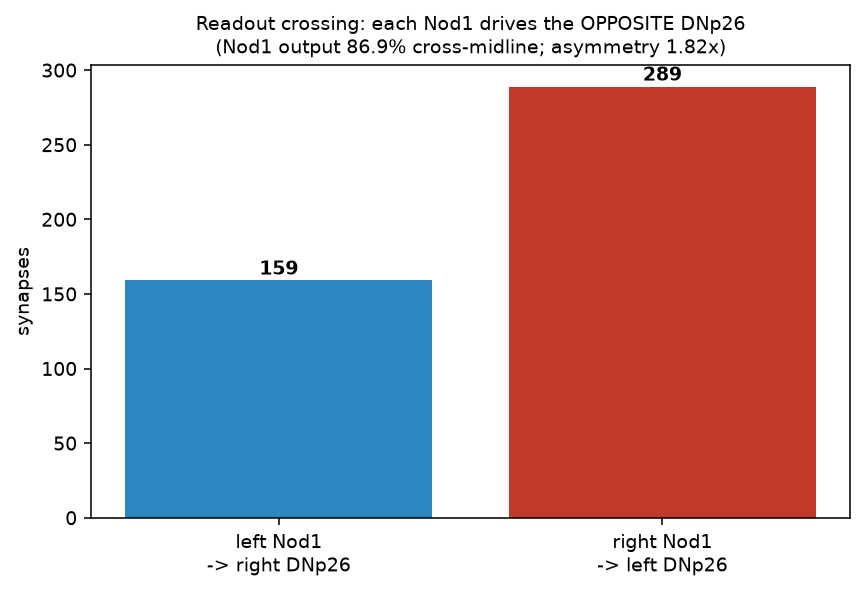
\includegraphics[width=0.75\textwidth]{figures/readout_crossing.png}
\caption{The readout crossing. Each side's Nod1 drives the opposite hemisphere's DNp26 steering
command, with the two directions unequal in strength.}
\label{fig:readout}
\end{figure}

\begin{figure}[t]
\centering
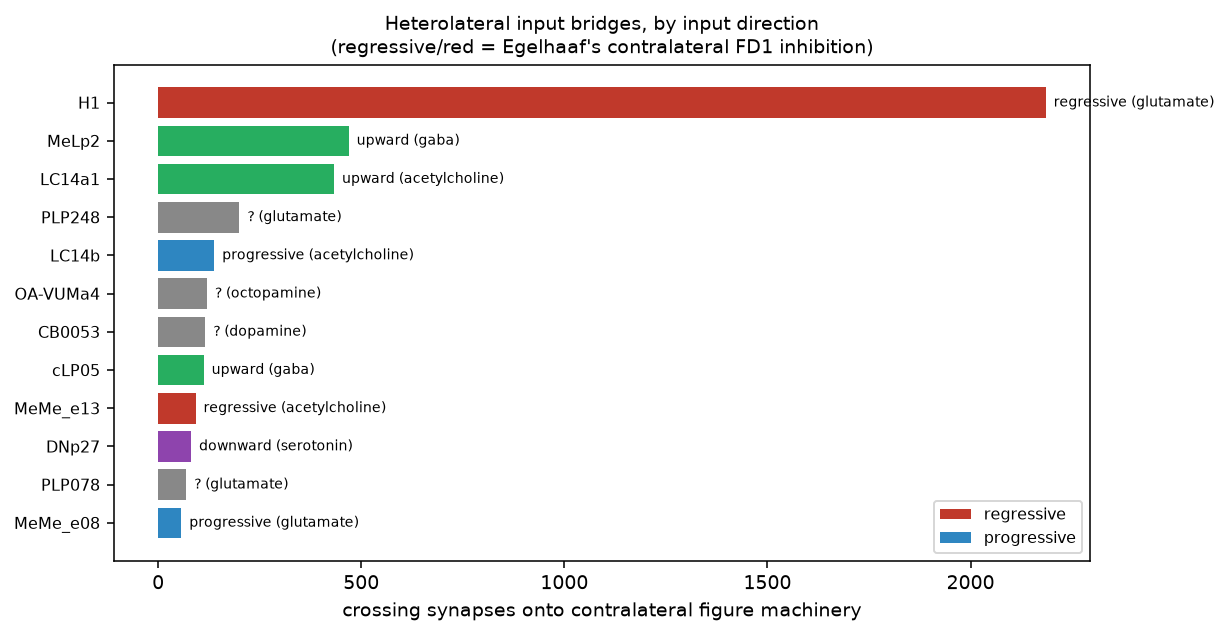
\includegraphics[width=0.92\textwidth]{figures/heterolateral_bridges.png}
\caption{Heterolateral input bridges onto the figure cells, colored by the motion direction of
their input. The dominant inhibitory bridge H1 reads regressive motion (red), matching Egelhaaf's
contralateral inhibition of FD1; weaker bridges read other directions.}
\label{fig:bridges}
\end{figure}

\begin{figure}[t]
\centering
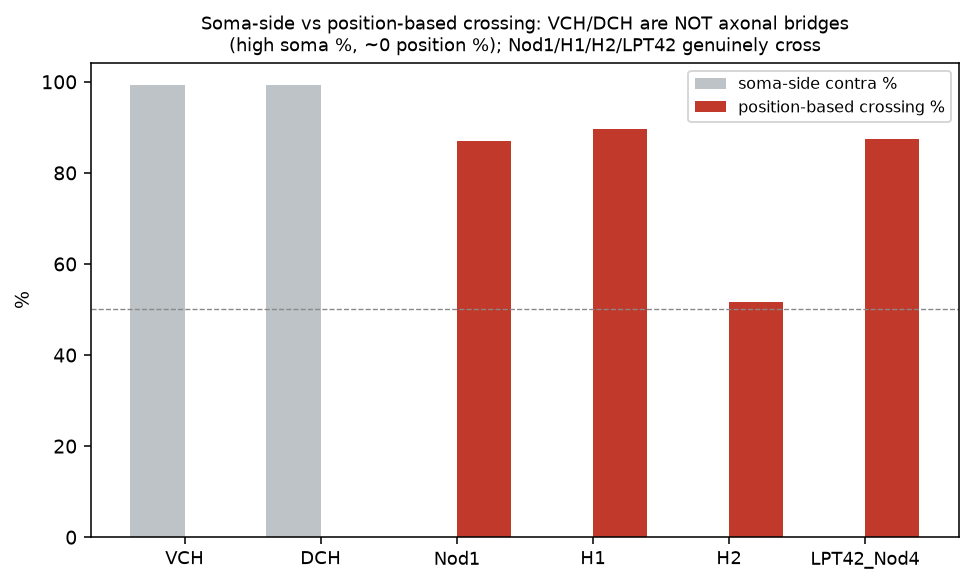
\includegraphics[width=0.85\textwidth]{figures/soma_vs_position.png}
\caption{The methodological result. By soma side, VCH and DCH appear 99 percent contralateral; by
synapse position they do not cross at all, because their soma and arbor are on opposite sides. The
genuine crossers Nod1, H1, H2, and LPT42\_Nod4 cross by both measures.}
\label{fig:somavspos}
\end{figure}

\begin{figure}[t]
\centering
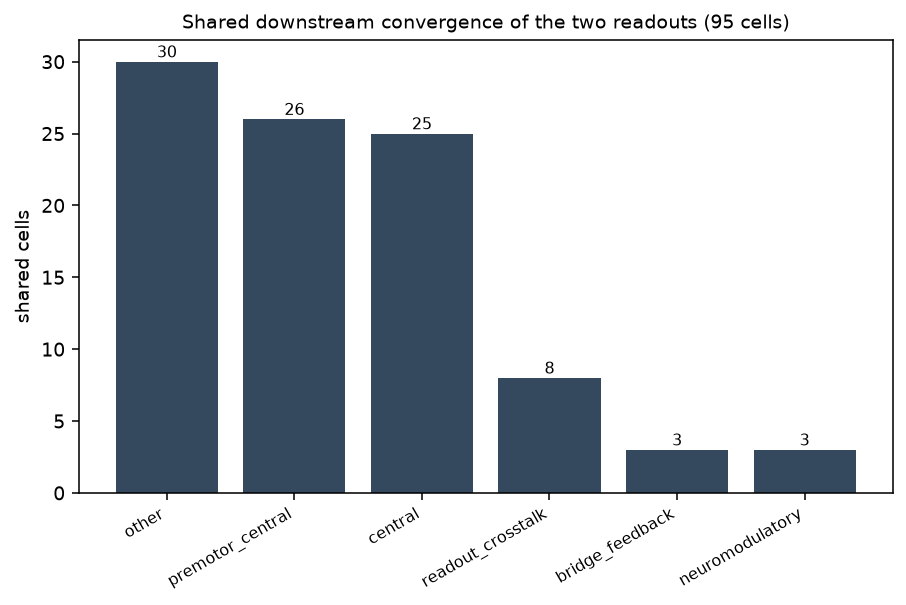
\includegraphics[width=0.8\textwidth]{figures/shared_convergence.png}
\caption{The shared downstream convergence. Cells receiving from both the left and right figure
readout, by role.}
\label{fig:shared}
\end{figure}

\section*{Data and reproducibility}

The analysis uses the public FlyWire FAFB connectome at materialization version 783, with chemical
synapses from \texttt{synapses\_nt\_v1} and no cleft-score threshold. A true inter-hemispheric
crossing is defined by synapse position relative to the synapse-space midline (\rid{529}
micrometres), validated by a fail-fast self-test that the two optic lobes separate cleanly. The
per-channel ledger, the named bridge manifest, and the figures are provided alongside this
document in the stage directory.

\end{document}
